\documentclass{beamer}
\usetheme{Madrid}

\usepackage{pifont}
\usepackage{amsmath}
\usepackage{xcolor}
\usepackage{graphicx}
\usepackage{subcaption}

\usepackage{xurl}

\usepackage{drawstack}
\usepackage{tikz}
\usetikzlibrary{decorations.pathreplacing}

% default path to images and other assets
\graphicspath{{assets/}}

% disable wrapping
\tolerance=1
\emergencystretch=\maxdimen
\hyphenpenalty=10000
\hbadness=10000

\DeclareMathOperator{\med}{med}

\newcommand{\rect}[1]{
  \begin{tikzpicture}
     \fill[#1] (0,0) rectangle (0.5,0.2);
  \end{tikzpicture}
}

% number figure caption
\setbeamertemplate{caption}[numbered]

% display bib label in references
\setbeamertemplate{bibliography item}{\insertbiblabel}
\setbeamertemplate{bibliography entry title}{}
\setbeamertemplate{bibliography entry location}{}
\setbeamertemplate{bibliography entry note}{}

% props and cons list items
\newcommand{\pros}{\item[{\textcolor[HTML]{3C8031}{\ding{51}}}]}
\newcommand{\cons}{\item[\textcolor{red}{\ding{54}}]}

% Databases
\newcommand{\wos}{\textit{Web of Science} }
\newcommand{\sco}{\textit{Scopus} }

% Metadata
% ------------------------
\title[Scientific metrics]{Scientific metrics}

\author[O. Shkalikov \and M. Zannini \and Q. Qaribiyan]
{Oleh Shkalikov \and Matteo Zannini \and Qader Qaribiyan}

\institute[]{TU Dresden, Computer Science Faculty}

\date{December, 2022}

% ------------------------

\begin{document}

\frame{\titlepage}

\begin{frame}
    \frametitle{Agenda}
    \tableofcontents
\end{frame}

\section{Simple metrics}

\section{Bibliometrics}

\begin{frame}
    \centering
    \Huge
    Bibliography metrics
\end{frame}

\subsection{Impact Factor}
\begin{frame}
    \frametitle{IF (Impact Factor)}
    \begin{block}{What is Impact Factor?}
        \textbf{Impact Factor}\cite{garfield1972citation} --- a per-year
        metric based on \wos database which reflect the mean number of citation
        to the paper published within prior 2 year.
    \end{block}

    The Impact Factor is calculated by the following formula:
    \[
        \text{IF}(y) = \frac{C(y)}{D(y - 1) + D(y - 2)}
    \]
    where
    \begin{itemize}
        \item $C(y)$ -- number of citation to the articles published in $[y-2, y-1]$~years
        \item $D(y)$ -- number of published articles in year $y$
    \end{itemize}
\end{frame}

\begin{frame}
    \frametitle{IF: advantages and disadvantages}
    \begin{columns}[T]
        \begin{column}{.5\textwidth}
            \centering \textbf{Pros}
            \begin{itemize}[<+->]
                \pros Easily calculated and interpreted
            \end{itemize}
        \end{column}
        \begin{column}{.5\textwidth}
            \centering \textbf{Cons}
            \begin{itemize}[<+->]
                \cons Limited availability
                \cons Lack of reproducibility
                \cons Doesn’t adjust for the distribution of citations
                \cons Windowed approach (especially 2 year window)
                \cons Doesn’t distinguish between citations made to articles, reviews, or editorials
                \cons Unstable
                \cons Doesn't allow to compare titles from different fields
            \end{itemize}
        \end{column}
    \end{columns}
\end{frame}

\subsection{CiteScore}
\begin{frame}
    \frametitle{CiteScore}
    \begin{block}{What is CiteScore?}
        \textbf{CiteScore}\cite{CiteScore2016} --- a per-year metric provided
        by \sco which measure rate between the received citations
        to \textbf{all peer-reviewed documents} of a title published within 4 years.
    \end{block}

    The CiteScore is calculated by the following formula:
    \[
        \text{CiteScore}(y) = \frac{CD_{y-3}(y)}
        {D(y) + D(y-1) + D(y-2) + D(y-3)}
    \]
    where
    \begin{itemize}
        \item $CD_x(y)$ -- the number of citations in year range from $x$ to $y$
              to all documents published within those years.
        \item $D(y)$ -- the number of all \textbf{peer-reviewed} documents published in year~$y$
    \end{itemize}

\end{frame}

\begin{frame}
    \frametitle{CiteScore 2016 vs CiteScore 2019}
    \begin{alertblock}{CiteScore 2019-2021 vs CiteScore 2016-2018}
        Previously CiteScore has been calculated within 3 year range, and count
        citation received only in year $y$.
    \end{alertblock}

    \[
        \text{CiteScore} = \frac{\sum \mathord{\rect{orange}}}{\sum \mathord{\rect{cyan}}}
    \]

    \begin{columns}[T]
        \begin{column}{.5\textwidth}
            \begin{figure}[ht]
                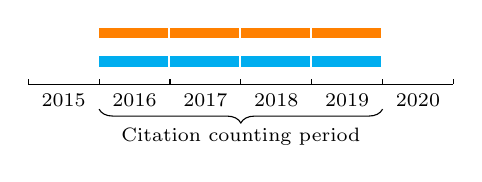
\begin{tikzpicture}[
                        scale=0.9,
                        every node/.style={
                                font=\scriptsize,
                                text height=1ex,
                                text depth=.25ex,
                            },
                    ]

                    \draw[-] (0,-0.4) -- (6,-0.4);

                    \foreach \x in {0,1,...,6}{
                            \draw (\x cm,-0.33) -- (\x cm,-0.4);
                        }

                    \foreach \x in {1,2,...,4}{
                            \fill[orange] (\x,0.25) rectangle (\x - 0.025 + 1,0.4);
                        }

                    \foreach \x in {1,2,...,4}{
                            \fill[cyan] (\x,0) rectangle (\x - 0.025 + 1, -0.15);
                        }

                    \node[anchor=north] at (0.5,-0.4) {$2015$};
                    \node[anchor=north] at (1.5,-0.4) {$2016$};
                    \node[anchor=north] at (2.5,-0.4) {$2017$};
                    \node[anchor=north] at (3.5,-0.4) {$2018$};
                    \node[anchor=north] at (4.5,-0.4) {$2019$};
                    \node[anchor=north] at (5.5,-0.4) {$2020$};

                    \draw[decorate,decoration={brace,amplitude=5pt}] (5,-0.75) -- (1,-0.75)
                    node[anchor=north,midway,below=4pt] {Citation counting period};
                \end{tikzpicture}
                \caption{CiteScore 2019}
            \end{figure}
            \rect{orange} -- number of citation received \\
            by publications published in citation counting period
        \end{column}
        \begin{column}{.5\textwidth}
            \begin{figure}[ht]
                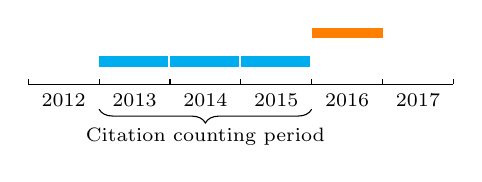
\begin{tikzpicture}[
                        scale=0.9,
                        every node/.style={
                                font=\scriptsize,
                                text height=1ex,
                                text depth=.25ex,
                            },
                    ]

                    \draw[-] (0,-0.4) -- (6,-0.4);

                    \foreach \x in {0,1,...,6}{
                            \draw (\x cm,-0.33) -- (\x cm,-0.4);
                        }

                    \fill[orange] (4,0.25) rectangle (5, 0.4);

                    \foreach \x in {1,2,...,3}{
                            \fill[cyan] (\x,0) rectangle (\x - 0.025 + 1, -0.15);
                        }

                    \node[anchor=north] at (0.5,-0.4) {$2012$};
                    \node[anchor=north] at (1.5,-0.4) {$2013$};
                    \node[anchor=north] at (2.5,-0.4) {$2014$};
                    \node[anchor=north] at (3.5,-0.4) {$2015$};
                    \node[anchor=north] at (4.5,-0.4) {$2016$};
                    \node[anchor=north] at (5.5,-0.4) {$2017$};

                    \draw[decorate,decoration={brace,amplitude=5pt}] (4,-0.75) -- (1,-0.75)
                    node[anchor=north,midway,below=4pt] {Citation counting period};
                \end{tikzpicture}
                \caption{CiteScore 2016}
            \end{figure}
            \rect{cyan} -- number of documents (in CiteScore 2019 only peer-reviewed)
            published in corresponding year
        \end{column}
    \end{columns}
\end{frame}

\begin{frame}
    \frametitle{CiteScore: advantages and disadvantages}
    \begin{columns}[T]
        \begin{column}{.5\textwidth}
            \centering \textbf{Pros}
            \begin{itemize}[<+->]
                \pros Transparency
                \pros Only citation from peer-reviewed content counted
                \pros Covers more titles than IF
                \pros Easily calculated and interpreted
                \pros More robust and stable than IF
            \end{itemize}
        \end{column}
        \begin{column}{.5\textwidth}
            \centering \textbf{Cons}
            \begin{itemize}[<+->]
                \cons Bounded to the \sco database
                \cons Doesn’t adjust for the distribution of citations
                \cons Windowed approach
                \cons Doesn't allow to compare titles from different fields
            \end{itemize}
        \end{column}
    \end{columns}
\end{frame}

\subsection{SNIP}
\begin{frame}
    \frametitle{SNIP (Source Normalized Impact per Paper)}
    \begin{block}{What is SNIP?}
        \textbf{SNIP}\cite{moed2010measuring} measures a journal's contextual
        citation impact, taking into account subject field with use of, so called,
        citation potential of the field of science. The SNIP score is calculated based on
        \sco database.
    \end{block}

    The SNIP is calculated by the following formula:
    \[
        \text{SNIP}(y) = \frac{RIP(y)}{RDCP(y)}
    \]
    where
    \begin{itemize}
        \item $RIP(y)$ -- raw impact per paper in year $y$ (IPP / CiteScore 2016)
        \item $RDCP(y)$ -- relative database citation
              potential in a journal’s subject field in year $y$
    \end{itemize}
\end{frame}

\begin{frame}
    \frametitle{RDCP}
    \begin{columns}[T]
        \begin{column}{.5\textwidth}
            % \vspace*{20pt}
            \[
                RDCP^j(y) = \frac{DCP^j(y)}{\operatorname*{med}\limits_{i} \; {DCP^i(y)}}
            \]
            where DCP -- database citation
            potential in a journal’s subject field:
            \[
                DCP^j(y) = \frac{\sum\limits_{p \in CP(y)} DCP^j_p(y)}{\# CP^j(y)}
            \]
        \end{column}
        \begin{column}{.5\textwidth}
            \begin{figure}[ht]
                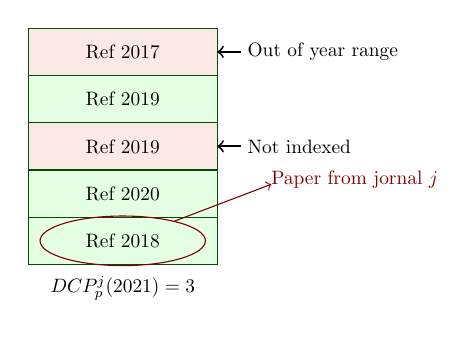
\begin{tikzpicture}[scale=0.6, every node/.style={scale=0.7}]
                    \bcell{Ref 2017} \cellptr{Out of year range}
                    \cell{Ref 2019}
                    \bcell{Ref 2019} \cellptr{Not indexed}
                    \cell{Ref 2020}
                    \cell{Ref 2018} \cellround{Paper from jornal $j$}
                    \cell[draw=none]{$DCP^j_p(2021) = 3$}
                \end{tikzpicture}
                \caption{Example of $DCP^j_p$ calculation}
            \end{figure}
        \end{column}
    \end{columns}
    where
    \begin{itemize}
        \item $CP^j(y)$ -- papers  citing the
              journal $j$ and \textbf{published in
                  journals processed for the
                  database} in the range $[y-3, y-1]$ years
        \item $DCP^j_p(y)$ -- number of references to the
              papers published in those years
              from paper $p \in CP^j(y)$
    \end{itemize}
\end{frame}

\begin{frame}
    \frametitle{SNIP: advantages and disadvantages}
    \begin{columns}[T]
        \begin{column}{.5\textwidth}
            \centering \textbf{Pros}
            \begin{itemize}[<+->]
                \pros Transparency
                \pros Only citation from peer-reviewed content counted
                \pros Covers more titles than IF
                \pros More robust and stable than IF
                \pros Allow to compare titles from different fields
            \end{itemize}
        \end{column}
        \begin{column}{.5\textwidth}
            \centering \textbf{Cons}
            \begin{itemize}[<+->]
                \cons Bounded to the \sco database
                \cons Hard to interpret
                \cons Calculation is more complicated
                \cons Citation potential tends to be highest for topical journals
            \end{itemize}
        \end{column}
    \end{columns}
\end{frame}

\subsection{SJR}
\begin{frame}
    \frametitle{SJR (SCImago Journal Rank)}
    \begin{block}{What is SJR?}
        \textbf{SJR}\cite{gonzalez2009sjr} is a metric provided by
        \sco which is based on the number of citations and the prestige
        of the titles which cite this journal.
    \end{block}

    Key points of SJR:
    \begin{itemize}
        \item Based on PageRank\cite{page1999pagerank} algorithm to calculate
              the prestige of the journal: citations issued by more important journals will be more valuable than those
              issued by less important ones
        \item Self-citation limited to 33\% of the total references
        \item Citation time frame is 3 year
    \end{itemize}
\end{frame}

\begin{frame}
    \frametitle{SJR: methodology}
    The SJR indicator is computed in two phases:
    \begin{enumerate}
        \item Prestige SJR (PSJR) -- size-
              dependent measure that reflects the overall journal prestige
        \item  normalization of this measure
              to give a size-independent metric
    \end{enumerate}

    The formula for the SJR metric (2 stage) is the following:
    \[
        \text{SJR}_i(y) = c \frac{PSJR_i(y)}{Art_i(y)}
    \]
    where
    \begin{itemize}
        \item $Art_i(y)$ -- number of primary items
              (articles, reviews, and conference papers) of journal $i$ published
              in three previous years [y-3, y-1].
        \item $c$ -- common constant to prettify values of SJR
    \end{itemize}
\end{frame}

\begin{frame}
    \frametitle{Prestige SJR}
    The PSJR calculation is an iterative process
    which started with \textbf{identical
        amount} of prestige to each journal until the differences
    between journal prestige in consecutive
    iterations is under threshold.
    \scalebox{0.84}
    {
        $
            PSJR_i = \overbrace{\frac{1-d-e}{N}}^{\text{min value}} +
            \overbrace{e \cdot \frac{Art_i}{\sum\limits_{j=1}^N Art_j}}^{\text{number of papers}} +
            \overbrace{d \left[ \sum\limits_{j=1}^N C_{ji} \cdot \frac{PSJR_i}{C_j} \cdot CF +
                    \frac{Art_i}{\sum\limits_{j=1}^N Art_j} \cdot \sum\limits_{k \in DN} PSJR_k \right]}^{\text{number and “importance” of the citations
                    from other journals}}
        $
    }
    where
    \alt<2>
    {
        \begin{itemize}
            \item CF(Correction Factor) is introduced that spreads the undistributed prestige
                  over all the journals proportionally to their accumulated prestige
        \end{itemize}
        \[
            CF = \frac{1 - \sum\limits_{k \in DN} PSJR_k}
            {\sum\limits_{h=1}^N \sum\limits_{l=1}^N C_{lh} \cdot \dfrac{PSJR_l}{C_l}}
        \]
    }
    {
        \begin{columns}[T]
            \begin{column}{.5\textwidth}
                \begin{itemize}
                    \item $C_j$ -- number of references of journal $j$
                    \item $C_{ji}$ -- references from journal $j$ to journal $i$
                    \item $d$ -- constant: $0.9$
                \end{itemize}
            \end{column}
            \begin{column}{.5\textwidth}
                \begin{itemize}
                    \item $N$ -- number of journals in the database
                    \item $DN$ -- journals that do not cite other journals
                    \item $e$ -- constant: $0.0999$
                \end{itemize}
            \end{column}
        \end{columns}
    }
\end{frame}

\begin{frame}
    \frametitle{SJR: advantages and disadvantages}
    \begin{columns}[T]
        \begin{column}{.5\textwidth}
            \centering \textbf{Pros}
            \begin{itemize}[<+->]
                \pros Transparency
                \pros Only citation from peer-reviewed content counted
                \pros Covers more titles than IF
                \pros Robust and stable
                \pros Self-citation is limited
                \pros Allow to compare titles from different fields
            \end{itemize}
        \end{column}
        \begin{column}{.5\textwidth}
            \centering \textbf{Cons}
            \begin{itemize}[<+->]
                \cons Bounded to the \sco database
                \cons Hard to interpret and calculate
                \cons Still windowed approach
            \end{itemize}
        \end{column}
    \end{columns}
\end{frame}

\section{Researcher's metrics}
\section{Researcher's metrics}
\begin{frame}
    \centering \Large Author-level metrics
\end{frame}
\begin{frame}
    \frametitle{h-index}

    \begin{block}{What is the h-index?}
        The \textbf{h-index} is a measure used to quantify the cumulative impact and relevance of an individual’s scientific research output.\cite{h-index}
    \end{block}

    \begin{alertblock}{}
        First introduced by Professor Jorge E. Hirsch in 2005.
    \end{alertblock}
    \textbf{h-index} formula:
    \[
        h = max(i ϵ Ν:f(i)>=i)
    \] \\
    where
   \centering i is the published paper and f(i) is the number of citations for i
    \begin{figure}[h]
        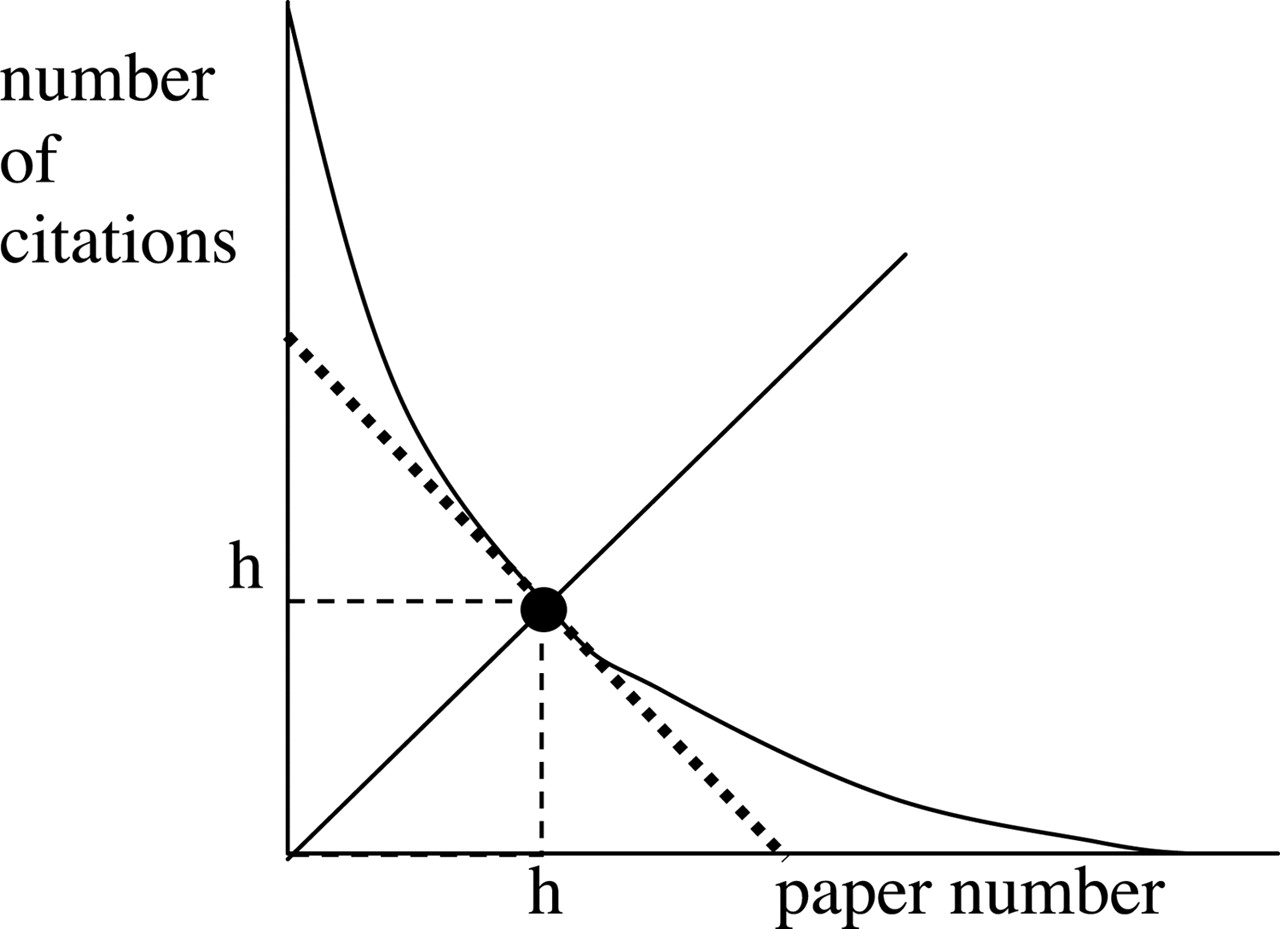
\includegraphics[height=0.3\textheight]{h-index_plot2.png}
        \caption{Graphical representation of the h-index}
    \end{figure}
\end{frame}

\begin{frame}
    \frametitle{h-index}

    \begin{exampleblock}{Example}
        \centering 4 publications:   A,B,C,D \hspace{0.5cm}   citations per paper:  7,5,4,3\\
        \centering h-index=3

    \end{exampleblock}
    \begin{columns}[T]
        \begin{column}{.5\textwidth}
            \centering \textbf{Pros}
            \begin{propslist}
                \item It avoids previous indexes' problems
                \item It measures both productivity and impact
                \item High h-index=high number of papers and citations
            \end{propslist}
        \end{column}
        \begin{column}{.5\textwidth}
            \centering \textbf{Cons} % example how to center one block
            \begin{conslist}
                \item Field of research is ignored
                \item Order of authors' contribution is ignored
                \item Insensitive to highly cited publications
                \item Exposed to manipulation
                \item Time-dependent
            \end{conslist}
        \end{column}
    \end{columns}

\end{frame}
\begin{frame}
    \frametitle{h-index variations}
    \begin{block}{m quotient}
        It allows comparisons between scientists with different career lengths.
    \end{block}\\
    \textbf{m quotient} formula:
    \[
        m = h/n
    \]
   \centering h: h-index, n: years of academic activity.

    \begin{block}{normalized h-index}
        It reduces the discipline bias.
    \end{block}
    \textbf{normalized h-index} formula:
    \[
      |h|=\frac{h}{d}
    \] where \centering h is the h-index and d the average number of academics in the field.
\end{frame}
\begin{frame}
    \frametitle{h-index variations}
    \begin{block}{individual h-index or hl}
        It reduces the effects of co-authorship.
    \end{block}
    \textbf{hl} formula:
    \[  hl = \frac{h}{\sum\limits_{i=1}^n a_i}\]
 where   \centering h is the h-index, n the number of papers and a_i \text{average number of authors.}
\end{frame}
\begin{frame}
    \frametitle{g-index}
    \begin{block}{What is the g-index?}
        The \textbf{g-index} is a modified version of the h-index
    \end{block}
    \begin{alertblock}{}
        First introduced by Leo Egghe in 2006.
    \end{alertblock}
    \begin{block}{How is it calculated?}
        Decreasingly order the papers based on the number of citations for each. The index is the largest number s.t. the top g articles received together at least g^2 citations.\cite{g-index}
    \end{block}\\
\end{frame}
\begin{frame}
    \frametitle{g-index}
    \textbf{g-index} formula:
    \[
       \centering  g^2 = \sum\limits_{i=1}^g c_i
    \]
  where  \centering c_i: \text{number of citations for each i paper.}\\
    \begin{figure}[g]
        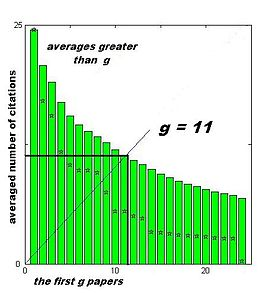
\includegraphics[height=0.3\textheight]{g-index_wiki.jpg}
        \caption{Graphical representation of the g-index}
    \end{figure}
\end{frame}

\begin{frame}
    \frametitle{g-index}
    \begin{exampleblock}{Example}
        \centering Top publications: 5\\
        \centering Citations:        25\\
        \centering g-index=5
    \end{exampleblock}
    \begin{alertblock}{}
        g is always greater or equal to h.
    \end{alertblock}
    \begin{columns}[T]
        \begin{column}{.5\textwidth}
            \centering \textbf{Pros}
            \begin{propslist}
                \item All h-index advantages
                \item It rewards papers with many citations
            \end{propslist}
        \end{column}
        \begin{column}{.5\textwidth}
            \centering \textbf{Cons} % example how to center one block
            \begin{conslist}
                \item Saturation value
                \item It lacks discriminatory power
                \item It only favours academics with many publications
            \end{conslist}
        \end{column}
    \end{columns}
\end{frame}

\begin{frame}
    \frametitle{c-indexes}
    \begin{block}{What are c-indexes?}
        \textbf{c-indexes} are the result of the augmentation of the h-index based on the citation order. \cite{c-index}
    \end{block}
    \begin{alertblock}{}
        Introduced in 2018 in the magazine Cureus.
    \end{alertblock}
    \textbf{c-indexes} formulas:
    \[
       \centering  c_p = h + i_p  \hspace{0.5cm}  c_s = h + i_s \hspace{0.5cm}  c_o = h + i_p + i_s
    \]
    The augmentations are given by the following formulas:

\centering \color{blue} i_p = $n_f$ + $0.5n_s$

\centering  i_s = $n_l$+ $0.5n_s$
    \end{frame}
    \begin{frame}
    \frametitle{c-indexes}
    \begin{columns}[T]
        \begin{column}{.5\textwidth}
            \centering \textbf{Pros}
            \begin{propslist}
                \item All the advantages of the h-index
                \item More accurate
                \item Takes citation order into account
            \end{propslist}
        \end{column}
        \begin{column}{.5\textwidth}
            \centering \textbf{Cons} % example how to center one block
            \begin{conslist}
                \item Time-dependent
                \item Field of research is ignored
            \end{conslist}
        \end{column}
    \end{columns}
\end{frame}
\begin{frame}
    \frametitle{l-index}
    \begin{block}{What is the l-index?}
        The \textbf{l-index} is a bibliometric measure derived from the h-index which enhances highly cited papers.\cite{l-index}
    \end{block}
    \begin{alertblock}{}
        Introduced in 2014.
    \end{alertblock}
    \textbf{l-index} formula:\\
    \centering given x real citation distribution, x* ideal citation distribution, C_x  \text{total number of citations}:\\
     \[
\centering L(x) = \sum\limits_{i=1}^n (\frac{1+x_i}{x_i*})x_i* \]
\centering After normalization:
\[
\centering  l(x) = \sqrt{\frac{L(x)}{ln2}}
    \]
\end{frame}
\begin{frame}
    \frametitle{l-index}
    \begin{columns}[T]
        \begin{column}{.5\textwidth}
            \centering \textbf{Pros}
            \begin{propslist}
                \item All the advantages of the h-index
                \item It rewards papers with many citations
                \item Regular and robust
            \end{propslist}
        \end{column}
        \begin{column}{.5\textwidth}
            \centering \textbf{Cons} % example how to center one block
            \begin{conslist}
                \item Time-dependent
                \item Order of authors' contribution is ignored
                \item Field of research is ignored
                \item Complex calculation
            \end{conslist}
        \end{column}
    \end{columns}
\end{frame}
\begin{frame}
\frametitle{CONCLUSION}
\begin{itemize}
\item [$\blacksquare$] Simple metrics like number of publications, number of citations or impact factor are often inappropriate to quantify the impact of a journal or an academic.
\item [$\blacksquare$] More complex metrics must be employed.
\item [$\blacksquare$] Deciding which metric to use depends on its specific properties and on the academic context.
\end{itemize}
\end{frame}

\begin{frame}[allowframebreaks]
    \frametitle{References}

    \bibliographystyle{apalike}
    \bibliography{references.bib}

\end{frame}

\end{document}
